\chapter{Background and Key Principle}

\section{Overview of Audio Data Hiding}

\subsection {General Scheme}
Audio data hiding or audio watermarking is the process of embedding information into audio data. There are two phases in general: watermark embedding and watermark detection. For embedding, an information is embedded into a original audio signal, produced a watermarked audio signal. This signal is sent to many other source for consuming and might suffer from some kind of processing or attacks, which might degrade the audio quality or the embedded watermark's correctness. On the other hand, watermark detection uses a watermark detector to extract the inserted watermark.

Usually, the original signal is divided into frames with a fixed frame length, the reason for this action would be discussed later in the thesis. Watermark bits are embedded into those frames using embedding techniques. After that, all the frames would be combined together to create a watermarked audio data. Similarly, watermark detector also split data into frame with the same parameter framelength, and use an inverse version of embedding technique to extract watermark.

\subsection {Performance Evaluation}
The field of audio data hiding has been existed for about twenty years, resulting in a lot of different approaches. This section presents several important definition required for evaluating an audio data hiding method. Usually, perceptual evaluation of audio quality (PEAQ) is used to measure the sound quality of the watermarked signals. Bit detection rate (BDR) is used to measure the accuracy of watermarking detection process.
\subsubsection*{Perceptual evaluation of audio quality}
PEAQ is used to measure quality degradation in audio according to the objective difference grade (ODG) which ranges from −4 to 0. ODG indicates the sound quality of target signals as shown in Table \ref{tab:PEAQ}.


\begin{figure}
\begin{center}
\begin{tabular}{ | m{6cm} | m{1cm} | } 
\hline
Quality degradation & ODG \\ 
\hline
Imperceptible & 0 \\ 
\hline
Perceptible, but not annoying & -1 \\ 
\hline
Slightly annoying & -2 \\ 
\hline
Annoying & -3 \\ 
\hline
Very annoying & -4 \\ 
\hline
\end{tabular}
\caption{Quality degradation of sound and PEAQ (ODG).}
\label{tab:PEAQ}
\end{center}
\end{figure}


\subsubsection*{Detection accuracy}
Detection accuracy was measured by BDR, the ratio between the numbers of correct bits and total bits as follows.
\begin{align}
\mbox{BDR} = \frac{\mbox{number of correctly detected bits}}{\mbox{total number of bits}}
\end{align}

\subsection{Embedding Techniques}
\subsubsection*{Methods based on least significant bits}
Methods based on least significant bits are the most conventional and simple technique. Watermark is embedded into audio signals by substituting or
manipulating the LS-bits of audio samples according to watermark bits. Since LS-bits do
not have much effect to the quality of audio signal, the distortion caused by this method
is not severe, hence the watermark is inaudible to users. The other advantage is the high
bit rate, e.g., 44100 bps for audio signals with a sampling frequency of 44.1 kHz. However,
this method has a serious limitation with robustness, even against simple signal-processing
manipulation such as addition of white noise.


\subsubsection*{Methods based on spread spectrum}
Inspired from the concept used in spread spectrum (SS) communication, a number of
methods of audio data hiding based on spread spectrum have been proposed. The principle
is that the watermark is spread over the large bandwidth spectrum so that the energy in a
single frequency is very small and it can be undetectable. This also enables the watermark
to be easily detected even if there is interference on some frequencies.
\subsubsection*{Methods based on echo hiding}
The simplest method based on echo hiding embeds information into the host signal by
introducing an echo in the host signal, which is an annutated delayed version of the host
signal \cite{echohiding} The watermark is encoded by the delay time of the echo, e.g., two different
values of delay time are used to encode one watermark bit. The delay times are carefully
chosen so that the watermark is inaudible and recoverable. By optimzing the delay
time, adding the echo to the host signal essentially emphasizes the host signal, making it
perceived louder, hence the watermark is basically inaudible to human auditory system
(HAS)\cite{has}
\subsubsection*{Methods in transform domain}
Methods in transformed domain exploit advantages of simultaneous masking character-
istics of HAS to embed inaudible watermarks. It is easier to incorporate perceptual
knowledge into the embedding algorithm in transformed domain than in time domain. A
simple way of exploiting perceptual knowledge is to embed watermark into the mid-range
frequency component, since the low frequency components are more sensitive to noise
and the high frequency components can be remove without degrading the audio quality.
Also, many of the state-of-the-art compression techniques such as MP3\cite{mp3} work in the same
framework. Watermark can be adapted with the models to resist perceptual compression.

In general, quantization index modulation (QIM)\cite{qim} technique is used for embedding
watermark in transformed domain because of its good robustness and blind nature \cite{QIMtwice}.
The embedding rule is quite simple. Suppose that a watermark bit needs to be embedded
into a variable, QIM quantizes the value of this variable according to the corresponding
scale. The watermarked variable is transmitted and may suffer from noise. To detect, the
distance from the watermarked variable to its closet point in each scale are calculated and
the watermark bit is decided by choosing the bit corresponding to the scale with the lower
distance. When applied to audio watermarking, QIM needs to specific acoustic features,
e.g., magnitude spectrum or phase spectrum, for embedding and reasonable quantization
step size (the distance between two point in the scales).
\section{Audio Data Hiding based on Phase Modification}
\subsection{Phase characteristic of audio signal}
To clearly understand the phase characteristic of audio signal, it's best that we first examine the phase of a single frequency sound. The below sinusoid function is the mathematic model for it:
\[s(t)=\cos{(2\pi ft+\phi)}\]
where f is frequency, φ is initial phase, and t is time variable. We may easily observe that
s(t) changes with the increase or decrease of φ, but the change pattern of s(t) is hard to
imagine. To see the point more clearly, we slightly modify the function of s(t) as follows.
\[s(t) = \cos(2\pi f (t + t_0))\]
where \(t_0=\frac{\phi}{2\pi f}\). Now, it is obvious that with the increase of $\phi$, $s(t)$ shifts to the left hand-side, whereas $s(t)$ shifts to the right hand-side with the decrease of $\phi$ along the time axis. Thus, modifying the phase of a pure-tone signal actually makes it come earlier or later in time domain. By extending this principle for a complex tone or a realistic audio-signal which is composed of multiple frequency components, 
it turns out that modification of the phase spectrum is the process that delays or advances the waveforms of corresponding frequency-components. 

Human ears perceive sound by separating into group of frequencies; each of group
is perceived as a single frequency. This phenomenon is called frequency selectivity of
HAS. Moderately modifying phase of frequencies in a group in synchronization does not
induce perceptible distortion but when phase relation between components in one group is
changed, the timbre changes drastically, leading to perceptible distortion. Moore et al. \cite{moore}
demonstrated that human ears appear insensitive to relative phase when the frequency
components are resolved, but with the unresolved frequency components, human ears can
easily detect distortion due to changing relative phase.

In another study, Ozawa et al. \cite{ozawa} revealed that human ears is hardly sensitive to
the difference in phase between two complex tones in high frequency range whereas with
low frequency components, the ears can perceive the difference as timbre change. It is
generally believed that if the phase-modification is kept sufficiently small, it is difficult
for human ears to distinguish between the original sound and the modified sound \cite{aiba}.
Phase is more related to spatial information of sound, hence more important for real or
3D sound and less important for recorded sound \cite{yasi}\cite{yost}.

Since the human ears are less sensitive to the phase of sound than to the noise and the
phase is less affected by processing, these properties have been exploited for inaudible and
robust watermarking over the recent years\cite{dong}. The methods work by modify-
ing the phase of the original audio signal according one of two amounts of modification,
each one encoding a bit of information. That is, the watermark data is represented by a
phase shift in the phase of the host signal.
The original signal is firstly split into a series of short frames. Next, fast Fourier
transform (FFT) is applied to each frame, generating a phase spectrum and a magnitude
spectrum. Then, the phase spectrum is added with the phase response of an infinite
impulse-response (IIR) APF or is quantized by QIM; two APFs or two quantization step
sizes are pre-defined to represent for each bit. The amount of modification is specified in a
manner that the watermark does not induce severe distortion and resist signal-processing
operations. There are two types of watermarking methods developed using the phase
of host signal, namely phase-modulation based watermarking and phase-coding based
watermarking.

\subsection{Phase coding for watermarking}
In phase-coding approach, watermark is embedded into the phase spectrum of the host
signal by QIM technique. The phase is quantized to two pre-defined scales in which each
one represents for a watermark-bit (‘0’ or ‘1’). The QIM step-size which quantifies for the
amount of phase-modification is pre-determined by experimental analysis. The higher
QIM step-size results in higher robustness but less degradation of watermarked-signal
quality and vice versa.

\subsubsection*{Watermark embedding}

\begin{figure}
  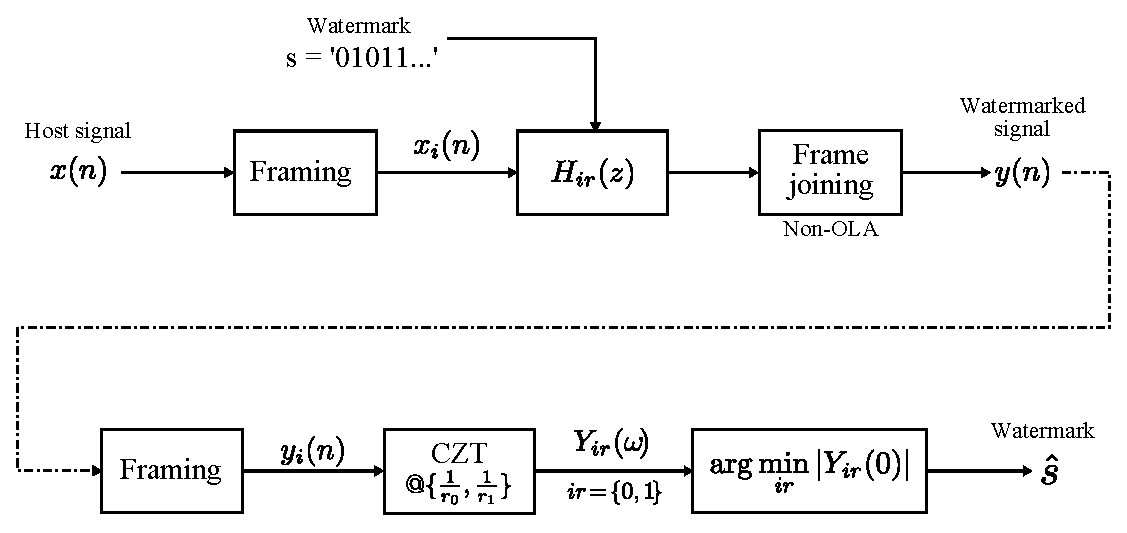
\includegraphics[width=1\textwidth]{PM_Scheme.eps}
  \caption{A scheme of audio data hiding based on phase coding: (a) watermark-embedding process and (b) watermark-detection process}
  \label{fig:pmscheme}
\end{figure}
The embedding process starts with frame segmentation of the host signal, \(x(n)\) into frames
\(x_i(n)\). Each watermark-bit from watermark \(s\) is embedded into one frame.

Figure \ref{fig:pmscheme} depicts a block diagram of the watermark-embedding process. A watermark-bit is em-
bedded into an audio frame as follows.
\begin{itemize}
\item{\textbf{Step 1.}} Original frame \(x_i(n)\) is transformed into the Fourier spectrum \(X_i(\omega)\) by FFT.
Magnitude spectrum \(|X_i(\omega)|\) and phase spectrum \(\angle X_i(\omega)\) are calculated.
\item{\textbf{Step 3.}} The watermark-bit are encoded into the phase of frequency-components by
QIM encoder and a quantized phase spectrum \(\angle Y_i(\omega)\) is obtained. Although each bit
can be embedded in only one component, it is embedded in all components to increase
robustness.
\item{\textbf{Step 3.}} The magnitude spectrum, \(|X_i(\omega)|\) and the quantized phase spectrum, \(\angle Y_i(\omega)\),
are combined into Fourier spectrum \(Y_i(\omega)\) and is then transformed into time domain signal
\(y_i(n)\) by inverse fast Fourier transform (IFFT).

\end{itemize}
Finally, all the processed frames are combined together to yield a watermarked signal
\(y(n)\).

\subsubsection*{Watermark detection}
The detection process also starts with frame segmentation of the watermarked signal,
\(y(n)\) into frames \(y_i(n)\). A Watermark-bit is detected from a watermarked frame as follows.

\begin{itemize}
\item{\textbf{Step 1.}} Watermarked frame \(y_i(n)\) is firstly transformed into \(Y_i(\omega)\) by FFT. Phase spectrum \(\angle Y_i(\omega)\)

\item{\textbf{Step 2.}} The phase of all frequency-components is decoded by QIM decoder all the bits. The output bit is determined by majority decision, e.g., if the number of `0' are greater the number of `1', the output is `0'.
\end{itemize}

These steps are repeated until we reach the final frame and all the watermark-bits are detected.
\section{Concurrency Programming}
\subsection{Basic concept}
Concurrency \cite{concurrency}is a concept comes from the field Communication Sequential Processes (CSP)\cite{csp}. In computer science, communicating sequential processes (CSP) is a formal language for describing patterns of interaction in concurrent systems. It is a member of the family of mathematical theories of concurrency known as process algebras, or process calculi, based on message passing via channels. 

Concurrency is the decomposability property of a program, algorithm, or problem into order-independent or partially-ordered components or units. This means that even if the concurrent units of the program, algorithm, or problem are executed out-of-order or in partial order, the final outcome will remain the same. This allows for parallel execution of the concurrent units, which can significantly improve overall speed of the execution in multi-processor and multi-core systems.

Large programs are often made up of many smaller sub-programs. For example, a web server handles requests made from web browsers and serves up HTML web pages in response. Each request is handled like a small program.

It would be ideal for programs like these to be able to run their smaller components at the same time (in the case of the web server to handle multiple requests). Making progress on more than one task simultaneously is known as concurrency. Go has rich support for concurrency using goroutines and channels.

\subsection{Golang}
Go\cite{golang} (often referred to as golang) is an open source programming language created by Google in 2007. It is a compiled, statically typed language in the tradition of Algol and C, with garbage collection, limited structural typing, memory safety features and CSP-style concurrent programming features added. The Go language has built-in facilities, as well as library support, for writing concurrent programs. Go introduces new concepts such as Goroutines and Channels to support concurrency programming. Those two are the basic blocks that made up our system.

\subsubsection*{Goroutines}
They're called goroutines because the existing terms—threads, coroutines, processes, and so on—convey inaccurate connotations. A goroutine has a simple model: it is a function executing concurrently with other goroutines in the same address space. It is lightweight, costing little more than the allocation of stack space. And the stacks start small, so they are cheap, and grow by allocating (and freeing) heap storage as required.

\subsubsection* {Channels}
Golang channels are pipelines to communicate between Goroutines. One Goroutine might has produced a value and want to send to other Goroutine, which would change behavior when receive this new value. This concept helps glue everything together and create a solid system of Goroutines working as a whole.

\begin{figure}
  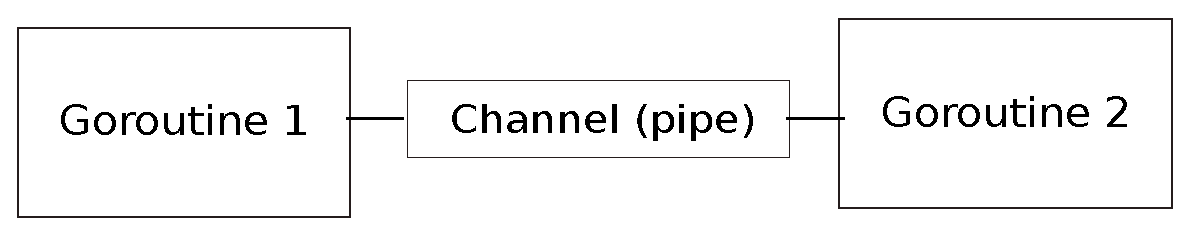
\includegraphics[width=1\textwidth]{goroutine.eps}
  \caption{Goroutines and channel}

\end{figure}